\documentclass[a4paper,10pt]{scrartcl}

\usepackage[english]{babel}

% Customizable sections
\usepackage{sectsty}

\usepackage{fancyhdr}
\fancyhead[R]{} %\includegraphics[height=2cm]{hw.pdf}}
\fancyhead[L]{{\sc F29OC Operating Systems and Concurency }}
 
\fancyfoot[L]{Hand-out: 12/02/2013}
\fancyfoot[R]{Hand-in:  26/02/2013}
\fancyfoot[C]{}
\pagestyle{fancy}

\renewcommand{\headrulewidth}{0pt}

\usepackage{graphicx}
\usepackage{hyperref}


\title{ 
    %{\sc F29OC Operating Systems and Concurency } \\
    Task 03
}
\date{}

\begin{document}
    \maketitle
    \thispagestyle{fancy}

    \section*{General requirements}
    Please submit the assignment as a \verb|*.zip| archive, where every
    problem is stored in its own subdirectory.  All the code must be
    well-commented and must come with a Makefile which builds a program.
    Notes and explanations may come in a separate file in the problem's
    directory.  For notes and explanations use text or pdf format.

 
    \section{Problem 1.1}
    Write your own memory allocator.  It doesn't have to be outrageously
    complicated, however it should work.  The allocator has to provide
    the standard interface for \textit{malloc} and \textit{free} so that it can be used 
    instead of system libc.  \textit{\small Preferably it should come
    as a static library.}

    %The memory allocator is allowed to use \textit{sbrk} call te
    
    \textsl{Some hints:}  

    \begin{description}
        \item[Allocator basics]
        Use the \textit{sbrk} system call to increase the data segment of
        the current process.  A call of the form \textit{sbrk(0)} returns the
        current program break; subsequent calls \textit{sbrk(N)}
        increase the program break by N bytes and return the last
        valid address. Check the manual pages for details.
        The space between these two addresses
        should be used to accommodate dynamic memory allocations.

        \item[Algorithm]
        Do use a linked list to administrate your allocator and store 
        the nodes of your linked list adjacent to the allocated memory.

        The easiest way to implement this is to simply prefix the
        chunks of allocated memory, i.e. portions of the memory received from
        sbrk that you reserve for it, with the size of reserved space and 
        a flag that indicates whether the chunk has yet been freed or not.

        The chunk-prefix structure could look like this:

        \begin{verbatim}
            struct chunk_info {
                size_t sz;
                int on;
                ...
            }
        \end{verbatim}

        With this structure, the memory allocation after \textit{malloc (n)},
        \textit{malloc (m)} would look like:
       

        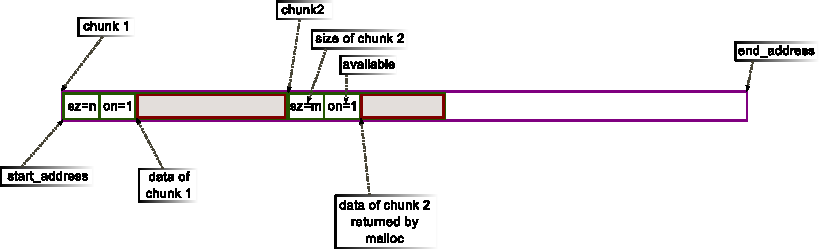
\includegraphics[width=.9\textwidth]{task-03-pic.pdf}

        Every time \textit{malloc(x)} is called, we save a chunk of
        memory of size $x$ + \textit{sizeof (struct chunk\_info)} bytes at some
        address $A$.  Please note that malloc should return 
        $A$ + \textit{sizeof (struct chunk\_info)} to a user.  

        Every \textit{malloc} call may require a traversal through all the
        chunks which is easy to implement -- we start with
        \verb|start_addr| which points to the first chunk.
        The next chunk can be accessed by stepping forward by
        
        \verb|(struct chunk_info*)start_addr->sz + sizeof (struct chunk_info)|
        
        bytes.  Subsequent chunks can be accessed in a similar manner.

        There are many different ways how freeing can be implemented.
        The easiest would be to
        set \verb|on| field to \textit{0}.

        If no suitable space can be found \textit{malloc} needs to return
        \textit{NULL}.

    \end{description}

    Use only one \textit{sbrk} call to get up to 1 GB of memory.


    \section{Problem 1.2}
    Compare the behaviour of your implementation with that of 
    \textit{malloc } implemented in
    your system's libc.  Find a use-case, where your implementation would
    exhaust the memory (although total size of allocated memory is less
    than 1 GB), but the system allocator would not.
    Describe the behavioural differences you can observe, provide
    some experimental evidence for your observations, and try to find out
    what is being done differently. 

    \textsl{Hint:}
    Create a simple program that performs a sufficiently long sequence of
    \textit{malloc} and \textit{free} calls so that you can experimentally observe
    this behaviour. You may also want to look into a small program that allocates
    several chunks and prints the addresses of the memory it has obtained.
    Feel free to use external materials to read up on memory allocators.
    

    \section{Problem 1.3}
    Think of the range of possible ways to overcome the fragmentation issues
    observed in 1.2.
    Improve your allocator by applying one or several of the techniques
    you can envision.
    The least you should do is to amalgamate adjacent free chunks into bigger ones.
    However, feel free to apply more more radical improvements to your allocator.
    The sky is the limit, be creative!
    
    \section{Problem 1.4}
    Compare your improved allocator with the previous one and with the 
    system allocator. Provide experimental evidence of the impact of your
    improvement. Try to come up with further ideas for improvement and
    further tests that exhibit a potential difference in behaviour.

    Besides memory fragmentation, consider aspects such as the time needed for
    \textit{malloc} or \textit{free} calls or the ability to be called in 
    a multi-threaded context.

    \textsl{Hints:}
    Measure the time it takes to perform $10^6$ mallocs interleaved with
    some random frees.  The program \verb|malloc-tester.c| will help you 
    to do that.  Measure the program against system memory
    allocator and memory allocators from problem 1.2 and 1.3.
    
    \section{Problem 1.5}

    Find out what a real system 
    allocator is doing differently by looking at any existing
    implementation. Describe the design decisions taken and try to
    explain why.

    Advice: take something reasonably simple like NetBSD/OpenBSD/...
    implementations.  However, if you are a real jedai, go for GNU
    libc implementation.

    Where to find these allocators?
    \begin{description}
        {\small
        \item[NetBSD]    
        \url{http://cvsweb.netbsd.org/bsdweb.cgi/src/lib/libc/stdlib/malloc.c}

        \item[OpenBSD]
        
        \url{http://www.openbsd.org/cgi-bin/cvsweb/src/lib/libc/stdlib/malloc.c}

        \item[Glibc (**)]
        
        \url{http://sourceware.org/git/?p=glibc.git;a=blob;f=malloc/malloc.c}
        }
    \end{description}

    In order to understand what is happening in the allocator follow the
    function calls that the allocator makes starting from
    \textit{malloc}.  In case of NetBSD, you may want to start with the
    \verb|malloc_bytes| function.  See what kind of structures are
    involved.

\end{document}
